
\documentclass{IEEEtran}
\IEEEoverridecommandlockouts
% The preceding line is only needed to identify funding in the first footnote. If that is unneeded, please comment it out.
\usepackage{cite}
\usepackage{amsmath,amssymb,amsfonts}
\usepackage{algorithmic}
\usepackage{graphicx}
\usepackage{textcomp}
\usepackage{xcolor}
\def\BibTeX{{\rm B\kern-.05em{\sc i\kern-.025em b}\kern-.08em
    T\kern-.1667em\lower.7ex\hbox{E}\kern-.125emX}}


\begin{document}

\title{Linux security modules and whole-system provenance capture\\
{\footnotesize}
\thanks{}
}

\author{\IEEEauthorblockN{ Aarti Kashyap} \\
\IEEEauthorblockA{\textit{Electrical and Computer Engineering} \\
\textit{ University of British Columbia}\\
Vancouver, Canada \\
kaarti.sr@gmail.com}


}

\maketitle

\section*{Abstract}
	 \textbf{Data provenance describes how data came to be in its present form. It includes data sources and the transformations that have been applied to them. There have been several different OS provenance capture tools in the past. However, only CamFlow and its predecessor Linux Provenance Modules use Linux Security Modules which is a  framework  that allows the Linux kernel to support a variety of computer security models while avoiding favouritism toward any single security implementation. This paper examines the relationship between LSM and CamFlow. the two key research questions that are addressed: 1) Does
	 the latest version of Linux LSM capture all security related information flows? 2) Given the results of (1) and the data captured by CamFlow in its LSM hooks, can we prove that an intrusion will be reflected as a different in the provenance graphs. This is an important question that either validates or refutes the use of kernel provenance for intrusion detection.}

\section{Introduction}
\label{What is provenance im general and with respect to computing?}

Provenance is the chronology of ownership, custody or location of a historical object. These documents are used to guide the authenticity and quality of an item. The term is used in a wide range of fields including science and computing. In computing...
\vskip 0.1in



Data provenance can help detect such intrusions in the kernel. Data provenance only provides with the capability to detect intrusions not prevent them. However, in order to make sure that all the intrusions are getting detected, we need a way to capture the complete data flow in the system which is why we chose to work with Camflow. 
\vskip 0.1in
\label{Camflow and whole system provenance and LSMs}

Camflow is a practical implementation of whole-system provenance capture that can be easily maintained and deployed. They use Linux security modules as the underlying framework to capture the data flows which provides us the ability to...


\label{What are we doing?}
In this paper, we examine if the whole system provenance capture mechanism developed by Camflow can be utilized for intrusion detection. 

\vskip 0.1in
\label{Applications of data provenance}

Data provenance has wide range of applications ranging from dependibility ( reliability and security) of the system to reproducibility of computational experiments.
\vskip 0.1in
\label{Role of data povenance in security}

Security is a major concern since there is no permanent fix to detect intrusions. Its a race between attackers and defenders.
An example to show that the kernel is still under threat Xioo et al (22) showed that attackers are able to manipulate the running behaviours of operating systems without injecting any malicious code. This type of an attack is called as kernel data attack. With the power of tampering data, the attackers can stealthily subvert various kernel security mechanisms. The 
\vskip 0.1in
\label{Challenge 1}

We first focus on a methodology proposed by Georget et al. to verify if indeed every security related flow goes through an LSM hook. The methodology proposed by Georget et al. had been designed for linux kernel v4.3 to ensure that all security flows are passing through the hooks. We gaurantee the same for v4.20 which is the last formal release. 
\vskip 0.1in
\label{Challenge 2}

A second challenge in determining if the use of kernel provenance can help in intrusion detection, we prove that a security breach is reflected in the provenance graph it produces. 
\vskip 0.1in

\textbf{Key contributions}

The key contributions of our work include: 1) analysing the callgraphs obtained from static analysis of the linux kernel to see if all paths are being tracked 2) a formalism to automate the process of analysing the callgraphs for the future versions 3)prove or disprove if indeed  


\section{Background and Objectives}
\begin{figure}
	\centering
	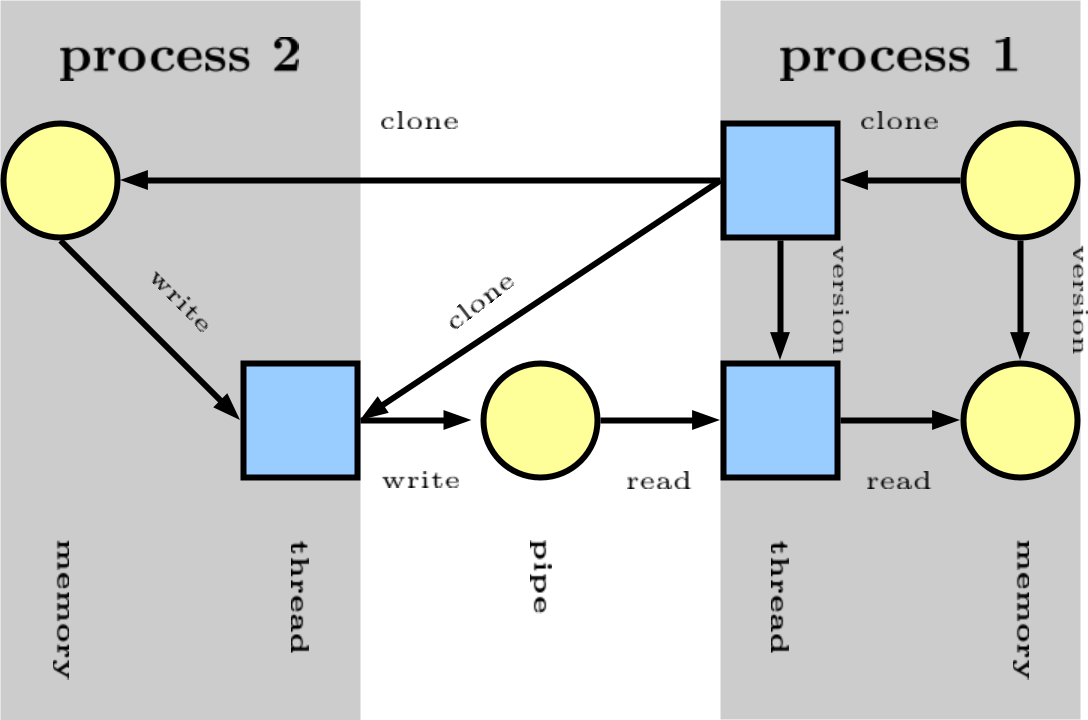
\includegraphics[width=0.7\linewidth]{graph}
	\caption[Provenance graph]{Process 1 clones process 2. Process 2 writes to a pipe. Process 1 read from the same pipe}
	\label{fig:graph}
\end{figure}
\begin{figure}
	\centering
	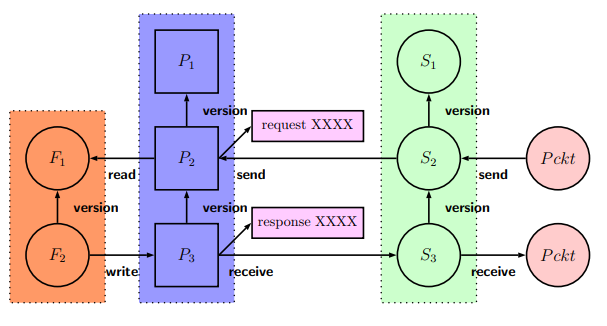
\includegraphics[width=0.7\linewidth]{Annotated-provenance-graph}
	\caption[Provenance graph]{Annotated provenance graph}
	\label{fig:annotated-provenance-graph}
\end{figure}

To provide context for the rest of the paper, we first introduce a few concepts. We introduce the notion of whole-system provenance, provenance graphs, Linux security modules and complete mediation property.

\subsection{Whole-system provenance capture}
\label{A little about the graphs}
Data provenance was originally introduced to understand the origin of data in a database. [17, 18] According to the W3C [19] standards provenance is defined as a directed acyclic graph (DAG). The vertices in the DAG represent entities(data), activities(transformations of data) and agents(persons or organizations). The edges represent the relationships between these elements. Mapping the graph definition to our system, which is the OS level entities are kernel objects, such as messages, network packets, files etc., but also xattributes, inode attributes, exec call parameters, network addresses, etc.
Activities are the tasks or processes carrying out manipulations on entities causing data flows. The agents are the persons or the organizations, who control the activities on different entities. These are the users and the groups at the OS level. 
 the agents are users and groups. Fig 1 illustrates these concepts. In the example in Fig 1, process 1 clones process 2. Process 2 writes to a pipe and finally process 1 read from the same pipe.
\vskip 0.1in 
Processes exchange information via system calls. Some system calls represent information exchange at some discrete point in time e.g, read, write; others may create shared states, e.g, nmap.


\label{A small recap into data provenance and whole system provenance capture}
\vskip 0.1in
There have been multiple whole system provenance capture systems proposed in the past such as HiFi[11], PASS[10]. However, they had a couple of problems: 1) struggled to keep abreast with current OS releases 2) Did not have whole system provenance capture guarantees 3) generated too much data 4)imposed too much overhead. Learning from the lessons from the past the whole system provenance capture systems, Camflow was introduced which promised to resolve all the above mentioned issues. Camflow addressed the above mentioned shortcomings 1) by leveraging the latest kernel defining to achieve efficiency 2) using a self-contained, easily maintainable implementation relying on Linux Security Modules, Net-filter, and other existing kernel facilities.


\subsection{Linux Security Modules}
\label{LSMs}
Since the kernel version 2.6, Linux added support for a framework to implement security extensions for the kernel called Linux Kernel Modules(LSM)(14). This framework provides a set of hooks strategically
placed in the kernel code associated with felds in internal data
structures for exclusive use by security extensions. The hooks are
functions which can be used by security extensions to (1), allocate,
free, and maintain the security state of various internal data structures having a dedicated security field, and (2), implement security
checks at specific points of execution, based on the security state
and a policy.  Security modules have a chance to apply security
restrictions anywhere a hook is present, but only at these places.
LSM’s original design is the access control and this has dictated the
placement of hooks in the code. . It is thus necessary to verify the
correctness of this placement for the purpose of information flow
tracking to ensure that information flow trackers. 
\vskip 0.2in
Since, Camflow uses LSMs and Net-Filters to capture the system provenance, the need to verify the correct placement of hooks for Camflow becomes necessary. 



\subsection{Complete Mediation Property}
The first goal of our contribution is to verify the property called "Complete Mediation property". According to this property for any execution path in the kernel starting with a system call and leading to an information flow, there is at least one LSM hook in the path which is reached before the flow is performed. It's important to verify this property. The reason is because if there exists a path generating a flow but not going through any LSM hooks, then there exists an opening for a malicious program to perform illegal actions without triggering any alarms. This is because information flow monitor can only react when one of the hooks is reached. 
\vskip 0.1in
In order to identify all the paths which lead to information flows requires solving two common problems in static analysis. The first problem is that the number of execution paths is infinite because of loops and recursions in the code. In order to finitize the code a subset is selected which should be sufficient to draw a conclusion for all the paths. In other words constructing an abstraction of the code which can be mapped to the concrete code after the analysis is required. The second problem  is that many execution paths that appear in the control flow graph (CFG) cannot actually be taken. These are called as the infeasible paths[20].  
\vskip 0.1in
For our analysis we consider all the system calls in the kernel version 4.20. Flow control requires knowing precisely when an information flow starts and when it stops. If this information is not available, it is not possible to maintain a correct representation of all flows currently taking place in the system at any given time. Since LSM was designed with access control in mind, some hooks might be missing to perform information flow tracking in every kernel update that comes. However, using static analysis we can find if some hooks are missing to perform information flow tracking. 
%\textbf{Georget et al methodology}
\vskip 0.1in
\label{Information flow}
The purpose of information flow control is to monitor the way in which information is disseminated in the system once it is out of its original container. This is unlike access control which can only enforce rules on how whose containers are accessed. Several scientific and technical challenges exist in ensuring complete information flow. One of them being the large Linux kernel code base. Georget et al.[3] tackles this issue in his work.

\vskip 0.1in
The most common way to meet the security objectives is access control. In order to ensure this, each level of security permissions is associated with the read or modifications of objects assigned to this level. This makes sure that only authorized users can read or alter information when stored in the object marked at the correct level of security. However, the fragility of this approach lies in the fact that once the information is out of their original container, the policy can no longer protect the information. To fully protect the information, the policy must be transitive. If Alice has access to a file but Bob does not, then we should make sure that Alice does not have some means to communicate with Bob. If Alice passes the information, even accidentally, then that is the violation of the confidentiality system.

\vskip 0.1in
The information flow control responds to the above problem. By keeping a track of information movement that took place between objects in the history of the system, it is able to protect information even when outside of its original container. This is not limited as the communications in the case of access control. As per the above Alice and Bob example, Alice has the right to contact Bob, until the knowledge to which Bob does not have access to is communicated. If that is indeed the case, then the communication has to stop. 

Hence, the initial Linux security module framework was built to support the access control mechanisms. We want to ensure that the framework is suitable enough to implement information flow mechanisms. 

%\label{Georget methodology}
%In order to improve the state of art of the information flow systems, Georget et. al developed a  plugin for the GCC compiler to easily extract and visualize control flow graphs of kernel functions...


\label{Camflow}
Camflow which utilizes LSM for the whole-system provenance capture. It collects the provenance data and constructs provenance graphs from the collected data. Now that we are aware that Georget's methodology ensures the placement of hooks such that complete information flow is possible, we show that the violations are reflected in the provenance graphs.


\begin{figure*}
	\centering
	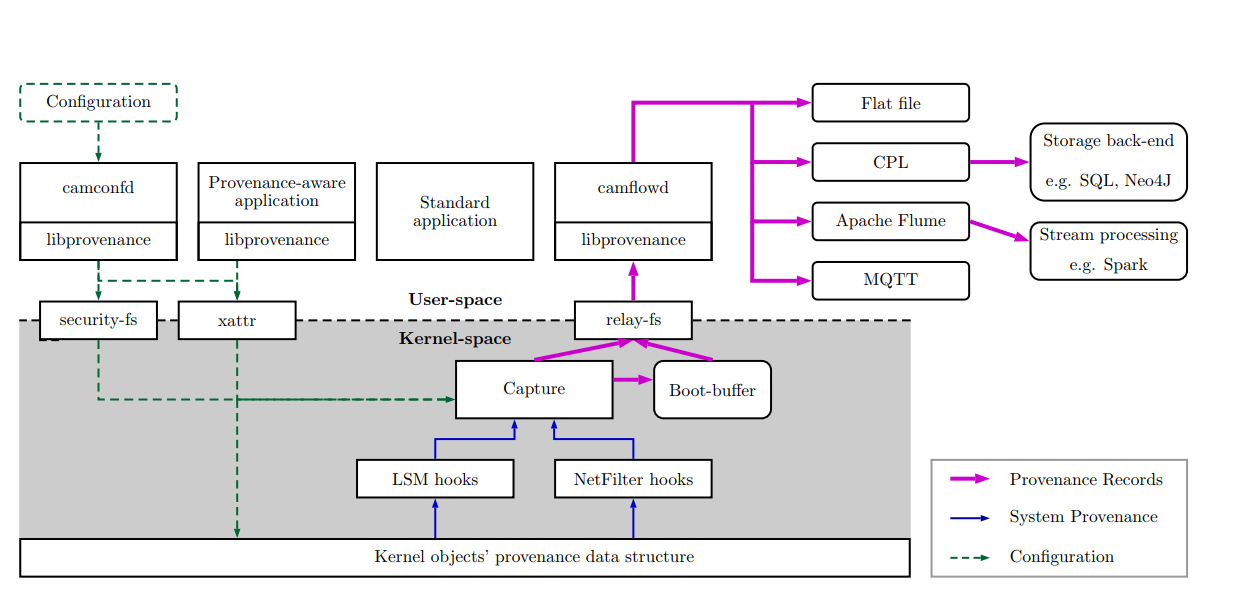
\includegraphics[width=0.7\linewidth]{camflow}
	\caption[Architecture overview]{Camflow architure}
	\label{fig:camflow}
\end{figure*}


\label{Introduction}
Though we have introduced what a Linux Security Module(LSM) means, we will discuss it in a little more detail. The Linux Security Module (LSM) framework provides a mechanism for various security checks to be hooked by new kernel extensions. The name “module” is a bit of a misnomer since these extensions are not actually loadable kernel modules. Instead, they are selectable at build-time via CONFIG\_DEFAULT\_SECURITY and can be overridden at boot-time via the "security=..." kernel command line argument, in the case where multiple LSMs were built into a given kernel.
\vskip 0.1in 
The primary users of the LSM interface are Mandatory Access Control (MAC) extensions which provide a comprehensive security policy. Examples include SELinux, Smack, Tomoyo, and AppArmor. In addition to the larger MAC extensions, other extensions can be built using the LSM to provide specific changes to system operation when these tweaks are not available in the core functionality of Linux itself.
\vskip 0.1in
Without a specific LSM built into the kernel, the default LSM will be the Linux capabilities system. Most LSMs choose to extend the capabilities system, building their checks on top of the defined capability hooks.





\section{Modeling the system calls causing flows}
The analysis technique we use if has been proposed by Georget et al. () for a subset of the system calls. It's a four step methodology which relies on the C compiler from the Gnu Compilers Collection(21). 

\begin{enumerate}
	\item The model designed by Georget to represent system calls and their execution paths does not describe the C source code. They instead use an internal representation called GIMPLE[]. 
	\item Each system call is represented by a control flow graph (CFG).
	\item The paths in these graphs model the execution paths in the program as defined by the classical graph theory[].
	\item The system calls are analysed one at a time. 
	\item Each system call contains multiple functions. These functions are inlined into the system calls to reduce the analysis to intra-procedural case. 
	\item Finally, in the CFGs, two kinds of nodes are marked: the nodes which correspond to the LSM hooks and the nodes which correspond to operation which generate the flows. 
	
\end{enumerate}

\subsection{Constraints in modelling}
In the CFGs which we construct , a node is not a basic block but a simple GIMPLE instruction. The analysis methodology does not deal with all expressions and variables of the language. Another reason for the same is that usage of floating-point values is explicitly prohibited in the Linux code. Variables representing structures or unions are also not handled when they involve pointer arithmetic. Global or volatile variables are also not handled, since they can have an arbitrary value at any point in the execution. Ignoring some variables does not hinder the soundness of
our approach: less impossible paths might be detected as such but
we never declare as impossible a possible path. A path in the CFG is said to be impossible when any execution
that would follow it would enter in an impossible state. For example,
a path including two conditional branching with incompatible
conditions would require a Boolean expression to be both true and
false at the same time. 



\section{Experience}



\section{Future work}3
\section{Limitations}
The limitations of our approaches are that we ignore the side channel attacks. We do not consider timing attacks. We restrict ourselves
to explicit information flows such as information storing or interprocess communications through means designed for this purpose.
We thus exclude covert channels and information leakage due to
some event or operation not occurring in the system.
\section{Related Work}
\section{Conclusion}
Hence, finally we run the analysis which was introduced by Georget et al[3] for the version 4.3 and we find three system calls which call LSM hooks but not all paths are mediated. These are listed in table 4 and 5.
\vskip 0.2in
We further provide a formalism to show that if all the flows pass through LSM hooks,then the flows gets captured by CamFlow. If they get captured by CamFlow, and assuming that no data is lost during the construction of the graphs, all the anomalies show up in the graphs.
\section{Future work}
The next step would be doing a similar analysis for the kernel version 5.x. Automating the technique to utilize the tools for the newer kernel version should be done. Georget et al.[3] provided a set of tools which when used, help in visualizing information flows, performing static analysis and finally getting to the results if any LSM hooks are missing. If we can automate this process for the future kernel versions, it will be a great contribution. 
\vskip 0.1in
Another contribution can be analysing the different IDS utilizing LSMs in different forms such as Blare, Weir, Laminar and understanding how and why they differ if they are utilizing the same underlying mechanisms. Is it just about the implementation or is there more to offer?
\vskip 0.1in
If indeed every action we perform shows up in a provenance graph, we can use that information to recreate information. I do mention this in the paper, however, proceeding in that direction sounds interesting. 
\vskip 0.1in
Another challenge would be to consider covert channels during the analysis.
\vskip 0.1in
I think health care could benefit a lot from such approaches. If we can have such concept in inside the human body, which creates a provenance of everything the body consumed. This is probably fiction for now, but maybe someday.



%
%
%
%
%\section{Introduction}
%System security is a race between the attackers and the defenders. The attackers adapt their attack model based on the defense mechanisms deployed on systems. The designers of the systems can build a completely correct system using formal methods such as theorem proving and model checking \cite{b4}. However, this only proves the correctness properties of the systems such as " Making sure that the system is following the correct protocol " or  " the shared memory allocation is done efficiently". The attacker can make sure that there is no violation in these properties and still manage to attack the system. In order to beat the attacker in this game, security-based mitigation techniques are proposed, which lack complete security coverage. \cite{b5}. Hence, in order to obtain a full or wider coverage of the system, using provenance-based techniques is an ideal way to proceed. \cite{b6}
%
%Provenance has many different definitions when used in different contexts. The simplest way to define provenance is a formal set of documents, to understand the beginning of something's existence and origin. These documents can be used to guide the authenticity or quality of the item. In a computing context, data provenance represents, in a formal manner, different relationships between entities (data items), activities (data transitions) and agents (which cause the transition). In other words, it can be understood as a formal set of documents which help in understanding the data existence and its flow to trace its integrity (quality). \cite{b1}
%
%Information flow tracking is a security mechanism designed to monitor how sensitive information spreads in a system. In data provenance context, information flow tracking is used to track the data and is be further used to put limits on the dissemination of a piece of sensitive data once it's out of its container of information. This allows high-level policies such as " my banking information will not be sent outside my system " or " my banking information will not be mixed with my wife's banking information" to be enforced easily.  \cite{b2}. Explicit information flow is defined as the copy, usually partial, of the content of one container of information to another. \cite{b3}
%
%Data provenance with a completeness property ensures that all the information flows of the data within the system are being recorded. Pasquier et. al \cite{b6} in his work on Run-time Analysis of Whole-system provenance ensures the completeness and accuracy of the provenance capture mechanism. He further makes use of Georget et al's \cite{b3} formalism to show that all the information flows between the kernel objects are properly recorded. However, this does not prove that all the security-related flows are also being captured by the system. This also does not tell us if the completeness of the information-flow property suffices to find intrusions.
%
%
%\begin{figure}
%	\centering
%	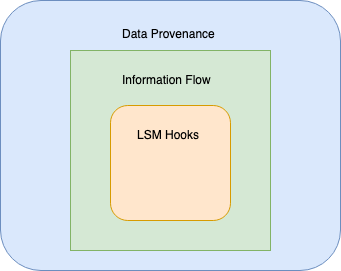
\includegraphics[width=0.7\linewidth]{Architecture-diagram}
%	\caption[]{High-level Architectural view. A structured way to formalize whole-system data provenance is to formalize if all the information flows are being captured. In order to make sure that all information flows are being captured we need to make use of LSM to insert hooks at every point in the kernel where a user-level system call is about to result in access to an important internal kernel object.}
%	\label{fig:architecture-diagram}
%\end{figure}
%
%
%
%
%
%
%
%Hence, as a part of this work we try to answer the question about complete and security-related information flows of the system using a whole-system provenance capture called Camflow.\cite{b7}
%
%The first part of the challenge includes answering the question if the completeness formalism is enough to detect all security related flows. Xueyuan et al. use a whole-system provenance capture tool for fault-detection \cite{b8}. Pasquier et. al. \cite{b6} shows that it's possible to detect intrusions during run-time of the system using CamFlow. However, is it enough to detect all sorts of data leaks and/or intrusions is one question we try to answer as a part of this work? This analysis has been performed for Linux Kernel 4.3. We try to see if the formalism still holds for the updated kernel version (5.0.x).
%
%The second contribution of our work is if indeed Camflow \cite{b7}  is able to capture all security-related flows, do they all show up as an anomaly in the provenance-graph. The provenance-graph is constructed from the data captured from all the security-related flows in the system. 
%
%
%\begin{figure}
%	\centering
%	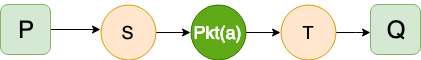
\includegraphics[width=0.7\linewidth]{DAG}
%	\caption{A simple provenance DAG: a process P sends packet Pkt(a) to process Q using the sockets S and T.}
%	\label{fig:dag}
%\end{figure}
%
%\section{Background}
%We conduct an analysis to see if the current version of the information flow patch applied to CamFlow is capable enough to catch all security violations. In order to do so, we make use of three open-source tools/libraries/patches CamFlow, GraphChi and complete flow capture formalism proposed by Georget et al \cite{b3}. 
%
%\subsection{CamFlow} 
%
%As we have discussed before data provenance records the chronology of ownership, change, and movement of an object or a resource. There are many provenance capture systems built before CamFlow such as PASS \cite{b10}, Hi-Fi\cite{b11} and Linux Provenance Module (LPM) \cite{b12}. However, none of the above mentioned Operating systems provenance capture systems utilize LSM except for it's predecessor LPM. LSM is a framework that allows the kernel to support a variety of computer security models while avoiding favoritism towards any of the security implementations. 
%
%We chose CamFlow for testing our hypothesis because it adopts the LSM architecture and support for NetFilters which makes it a maintainable practical whole-system provenance implementation.CamFlow maintains an information-flow patch based on Georget et al's \cite{b3}formalism which provides completeness guarantees. The fact that Cam-flow provides completeness guarantees, its a strong choice for researchers to use it as a fault-detection tool \cite{b8}. Pasquier et al. use CamFlow to perform a run-time analysis of whole-system provenance to find intrusions \cite{b6}. However, since the completeness guarantees are specific to kernel version 4.3, we want to provide a formalism which shows that it holds for the updated kernel versions.  
%
%In order to perform such an analysis,  Pasquier et al. have maintained a systematic build script for CamFlow Linux provenance.  This script generates kernel patch for CamFlow Linux provenance capture. It consists of two parts which are running the automated Travis script and  CircleCI script.  The Travis script 
%
%builds the kernel and eventually builds the kernel patch. The CircleCl script performs kernel analysis.
%
%\subsection{GraphChi}
%
%The representation of the provenance data is in the form of a directed acyclic graph (DAG). Every node in the DAG represents an entity, an activity or an agent. Each directed edge represents an interaction between each node. Fig.2 represents a simple example. In our context, entities are kernel objects, activities are tasks, and agents are users and groups. Fig 2 represents packet being sent from process P to Q from socket S to T. 
%
%We use GraphChi, a vertex-centric graph processing model to generate program models and to generate anomalies. The purpose of utilizing GraphChi is to answer that in case of security violations in the system, are the anomalies reflected in the graphs. This is a tool which we use for ensuring if all anomalies are reflected on the provenance graph after the capture. 
%
%
%\subsection{Formalism of complete mediation}
%
%Georget et al. \cite{b3} proposed a formalism to verify the property for complete capture of the information flows called \textit{Complete Mediation}. The authors use a compiler-assisted and reproducible static analysis on Linux kernel to verify that the LSM hooks are correctly placed with respect to operations generating information flows. This ensures that LSM-based information flow monitors can properly track all information flows.
%
%
%
%
%\section{Evaluation}
%
%The evaluation of the system is performed in two parts. The first part is where we focus on the completeness and accuracy of the current CamFlow patch with respect to the new kernel version. We also try to find if all the security-related flows are being captured by the LSM-interface. The second half of our evaluation focuses on the anomaly detection aspect. We want to prove ( or disprove ) if all security related flows are being captured by the LSM-interface, then the anomaly must show up in the provenance graph.
%
%\subsection{LSM interface and security-related flows}
%Before analysing if all security-related flows are being captured by the interface, we first ensure the sompletness and accuracy of the interface
%
%
%
%
%
%\subsubsection{Completeness}
%We want to ensure that all flows of information between kernel objects are properly recorded. The LSM framework \cite{b14} was originally implemented to support Mandatory Access Control (MAC) schemes but not information flow tracking. Georget et al \cite{b3} through static analysis of the kernel code base demonstrated that LSM framework is applicable to information flow tracking. By adding a small number of hooks it is possible to properly intercept all information flows between kernel objects.
%
%In order to run the analysis we use the scripts written by Pasquier et al \cite{b14} which generates the coverage, hooks, relations, stats and vertices for the system. We can see that some of the hooks such as the ones listed in Table 1 are ignored. The automated CircleCl script performs kernel source code analysis and generates the above mentioned attributes in the docs folder. 
%
%
%
%
%From the analysis we observe that the coverage is not complete. Hence, the attacker can still find ways to attack the system. The coverage for different system calls is different. For eg. we observe that for \_\_x64\_sys\_open system call the coverage is 8 out of 12. This means that out of the 12 hooks which were originally called by this system call, only 8 hooks were implemented. We observe similar coverage for different system calls. 
%
%\subsubsection{Security-related flows}
%Based on the coverage we observe a couple of security-related flows which will not be captured by the current provenance capturing mechanism.  If the attack is strictly about extracting information from within an application memory, the effect is not observed. 
%
%\subsection{Anomaly detection}
%Now that we are aware that some attacks are caught by the capture mechanism and there are some attacks which are not. We try to observe if all the attacks whose flow is being recorded by the capture mechanism if it is reflected on the graph. 
%
%From our evaluation, we understand that if the flow is being recorded it does get reflected on the graph. This is observed from the coverage analysis which we obtained from running the call graph scripts. However, currently, there is no formalism to prove so. So an important and very relevant contribution to this work would be to provide some form of formalism to show that this happens. Hence, my goal is to show some form of formalism before the final submission.  
%\section{Conclusion}
%
%After analyzing the results we observe a couple of things about CamFlow architecture, the formalism proposed by Georget et al. and finally about LSM. 
%
%The reason we performed this analysis was to observe the changes which will be required in the CamFlow code-base to make sure it adheres to the latest versions of the kernel. The other reason we carried out this analysis was how feasible is it to maintain CamFlow with respect to the latest kernel releases. The ultimate goal is to have provenance integrated into the mainline Linux kernel. Thus if we can keep up with the versions, it shows that CamFlow is a fully self-contained Linux kernel module. 
%
%Another observation from the results we can notice a clear completeness-security gap. This tells us that there is a lot more work to be done in order to build intrusion detection systems using provenance capture mechanisms. Provenance capture mechanisms can capture only a subset of the possible attacks.
%
%\section* {Discussion Topics}
%The first interesting discussion point is understanding the completeness-security gap if any. Currently, the DAGs are generated with respect to the provenance data. However, this is not taking the timing aspect into consideration. Provenance capture mechanisms currently are data related. The way we can capture anomalies is by learning the data pattern from previous immutable data. However, if the attacker brings in the timing aspect, keeping the data intact can that cause damage? It depends on the application if data delays can cause harm. 
%
%Another interesting point to discuss would be the completeness of information flows means that it guarantees that all flows are being captured. So you need to place hooks at the relevant places which ensures that all information flow paths are being recorded. However, again this does not cover the event aspect of the system. What if instead of modifying the data with alone or modifying the data with respect to time, it modifies the event in a smart way such that the correlations created by the DAG cannot spot it.  Instead of sending the data from process P to process Q, it sends it to process R. 
%\section*{Acknowledgment}
%
%This work was done as a part of our term project for CPSC 508. CPSC 508 is a graduate level operating systems course taken by Dr. Margo Seltzer.

\begin{thebibliography}{00}
\bibitem{b1} Lucian Carata, Sherif Akoush, Nikilesh Balakrishnan, Thomas Bytheway,
Ripduman Sohan, Margo Seltzer, Andy Hopper, an ``A Primer on Provenance,'' acmqueue, 2014.
\bibitem{b2} Daniel Crawl and Ilkay Altintas , A Provenance-Based Fault Tolerance Mechanism for
Scientific Workflows.

\bibitem{b3} Laurent Georget, Mathieu Jaume, Guillaume Piolle, ``Verifying the reliability of operating system-level information flow control systems in linux,'' Proceedings of the 5th International FME Workshop on Formal Methods in Software Engineering, FormaliSE ’17, pages 10–16, Piscataway, NJ, USA, 2017. IEEE Press.

\bibitem{b4}GERWIN KLEIN, ``Operating system verification—An overview,"Sadhan ¯ a¯ Vol. 34, Part 1, February 2009, pp. 27–69. © Printed in India

\bibitem{b5} Jonathan Pincus and Brandon Baker , ``Mitigations for Low-Level Coding Vulnerabilities:
Incomparability and Limitations ,'' 2004.


\bibitem{b6}Thomas Pasquier, Xueyuan Han, Thomas Moyer, Adam Bates, Olivier Hermant, David Eyers, Jean Bacon, Margo Seltzer, ``Runtime Analysis of Whole-System Provenance
,''16 pages, 12 figures, 25th ACM Conference on Computer and Communications Security 2018.



\bibitem{b7} Thomas Pasquier, Xueyuan Han, Mark Goldstein, Thomas Moyer, David Eyers, Margo Seltzer, Jean Bacon, Practical Whole-System Provenance Capture
, SoCC '17 Proceedings of the 2017 Symposium on Cloud Computing.


\bibitem{b8} Xueyuan Han, Thomas Pasquier, Tanvi Ranjan, Mark Goldstein, and Margo Seltzer, Harvard University

 , ``FRAPpuccino: Fault-detection through Runtime Analysis of Provenance ,'' HotCloud'17.



\bibitem{b9} PASQUIER, T. F.-M., SINGH, J., BACON, J., AND EYERS, D. , ``Information flow audit for paas clouds.
Cloud Engineering
(IC2E), 2016 IEEE International Conference on (2016), IEEE,
pp. 42–51.


\bibitem{b10} MUNISWAMY-REDDY, K.-K., HOLLAND, D. A., BRAUN, U.,
AND SELTZER, M. I. , `` Provenance-aware storage systems. ,'' In
USENIX Annual Technical Conference, General Track (2006),
pp. 43–56..


\bibitem{b11} POHLY, D. J., MCLAUGHLIN, S., MCDANIEL, P., AND BUTLER, K , ``Hi-fi: collecting high-fidelity whole-system provenance ,'' In Proceedings of the 28th Annual Computer Security Applications Conference (2012), ACM, pp. 259–268.


\bibitem{b12} Adam Bates, Dave (Jing) Tian, and Kevin R.B. Butler , ``Trustworthy Whole-System Provenance
for the Linux Kernel.
24th USENIX Security Symposium, 2015.








\bibitem{b13} PASQUIER, T. , ``Camflow information flow patch.
In https://github. com/CamFlow/information- flow- patch.
.


\bibitem{b14} 	Chris Wright,	
Crispin Cowan,	
Stephen Smalley,	
James Morris,	
Greg Kroah-Hartman.	
, ``Linux Security Modules: General Security Support for the Linux Kernel.
Proceeding
Proceedings of the 11th USENIX Security Symposium
Pages 17-31 

August 05 - 09, 2002 .


\bibitem{b15} PASQUIER, T. , ``CamFlow development.
In https://github.com/CamFlow/camflow-dev.

\bibitem{b16} INRIA , ``The Kayrebt Toolset
In http://kayrebt.gforge.inria.fr/


17 Peter Buneman, Sanjeev Khanna, and Tan Wang-Chiew. 2001. Why and where:
A characterization of data provenance. In International Conference on Database
Theory. Springer, 316–330.


18 Allison Woodruff and Michael Stonebraker. 1997. Supporting fine-grained data
lineage in a database visualization environment. In International Conference on
Data Engineering. IEEE, 91–102.

19 Khalid Belhajjame, Reza B’Far, James Cheney, Sam Coppens, Stephen Cresswell,
Yolanda Gil, Paul Groth, Graham Klyne, Timothy Lebo, Jim McCusker, Simon
Miles, James Myers, Satya Sahoo, Luc Moreau, and Paolo et al. Missier. 2013.
Prov-DM: The PROV Data Model. Technical Report. World Wide Web Consortium
(W3C). https://www.w3.org/TR/prov-dm/

20  Rastislav Bodík, Rajiv Gupta, and Mary Lou Soa. 1997. Refining Data Flow
Information Using Infeasible Paths. SIGSOFT Software Engineering Notes 22, 6
(Nov. 1997).

21 Richard Matthew Stallman and the GCC developer community. 2013. Using
the GNU Compiler Collection (GCC). Technical Report. https://gcc.gnu.org/
onlinedocs/gcc-4.8.4/gcc/
\end{thebibliography}




\end{document}
